\documentclass[a4paper,10pt,twoside]{report}

\usepackage{Packages}
\usepackage[framed,numbered,autolinebreaks,useliterate]{Listings}

\addto\captionsbritish{\renewcommand{\contentsname}{Table of Contents}}

%\linenumbers

\newcommand{\researchgroup}{Financial Computing 3}

\newcommand{\shortdoctitle}{Doc title}
\newcommand{\doctitle}{A Study of Deep Learning in Micro-Economic Analysis and Computational Finance}
\newcommand{\docsubtitle}{}

\newcommand{\authorone}{Zebo, Xiong}
\newcommand{\sauthorone}{Ph.D Student}
\newcommand{\authortwo}{XXX, XXX}
\newcommand{\sauthortwo}{Ph.D Student}
\newcommand{\keywords}{Finance, Deep Learning, Computation}
\newcommand{\version}{First version}
\newcommand{\monthYear}{December 2019}

\newcommand{\firstCommitteeMember}{Dr. Anxiao, Jiang}
\newcommand{\secondCommitteeMember}{}
\newcommand{\thirdCommitteeMember}{}

\author{\me}

\hypersetup
{
    pdfauthor   = {\authorone and \authortwo},
    pdftitle    = {\shortdoctitle},
    pdfsubject  = {\doctitle},
    pdfkeywords = {\keywords}
}

\begin{document}

\begin{titlepage}
\begin{center}

\includegraphics[height=2cm]{Figures/TAMU.png} \\
\LARGE
Texas A\&M University \\
\Large
Department of Computer Science \& Engineering \\
\large
\researchgroup

\vspace*{10cm}

\setlength{\TPHorizModule}{1mm}
\setlength{\TPVertModule}{\TPHorizModule}

\newlength{\backupparindent}
\setlength{\backupparindent}{\parindent}
\setlength{\parindent}{0mm}

\begin{textblock}{155}(32,89)
    \vspace*{1mm}
    \huge
    \textbf{\doctitle \\}
    \Large
    \vspace*{5mm}
    \textit{\docsubtitle} \\
    \vspace*{5mm}
    \Large
     \begin{tabular}{c c c}
            \authorone & \& & \authortwo \\
            \sauthorone & & \sauthortwo \\
    \end{tabular} \\
\end{textblock}

\large
Supervisors: \\
\begin{tabular}{c}
    \firstCommitteeMember \\
    \secondCommitteeMember \\
    \thirdCommitteeMember \\
\end{tabular}

\vfill
\version

\vfill
%\docdate \\
\large
College Station, \monthYear \\

\setlength{\parindent}{\backupparindent}
\end{center}
\end{titlepage} 

\normalsize

\chapter*{Abstract}\label{chapter:Abstract}
\setcounter{page}{0}
\pagenumbering{roman}
\addcontentsline{toc}{chapter}{Abstract}
During the last decades, computational methods gradually become the essential part of economy and finance researches. With the rise of attention on machine learning techniques, the investors and financial analyst realize the importance of utilize the computers' power to help them make critical business decisions and predict the future's trends.

\tableofcontents












\chapter{Collections}\label{chapter:Introduction}
This chapter collect the studies materials (including source from technology blogs, etc.) and technical information for the research 
\section{From Student}
\begin{enumerate}
    \item{Dive into paper "High-Frequency Factor Models and Regressions" 
        \begin{itemize}
         \item Un-systematic Risk (individual firm risk): Random events such as CEO step down, company being prosecuted, company news, etc; Systematic Risk (market wide risk): nationally cut interests rate, etc; 
         \item When portfolio size increase, the volatility will decrease because "Unsystematic Risk" averaging out.
         \item Total Risk = Systematic Risk + Unsystematic Risk
         \item How to measure Systematic risk? Beta
         \item Beta = the percentage change in an asset's return GIVEN a 1\% change in the market portfolio (market portfolio = all firms) - how individual return tied to market portfolio change
        \end{itemize}
        
    \item{Data from Thomson Reuters}
        \begin{itemize}
            \item Login Page:
                \begin{itemize}
                    \item  \url{https://php.library.tamu.edu/resources/datastream/} or 
                    \item  \url{http://eikon.thomsonreuters.com/login}
                \end{itemize}
            \item Credentials: 
                \begin{itemize}
                    \item   Account: student3@tamu.edu  | Password: TAMUwcl1
                    \item   Account: student2@tamu.edu  |Password: WCLtamu1
                    \item   Account: student1@tamu.edu  | Password: WCLtamu1
                \end{itemize}

        \end{itemize}
    
      \item{Data from Eikon Data API}
        \begin{itemize} 
           \item eikon PyPI  \url{https://pypi.org/project/eikon/}
           \item Quick Start  \url{https://developers.refinitiv.com/eikon-apis/eikon-data-api/quick-start}
           \item Tutorials
           \url{https://developers.refinitiv.com/eikon-apis/eikon-data-api/learning}
        \end{itemize}
        
     \item Sample Minutes Price (3 months) \\
            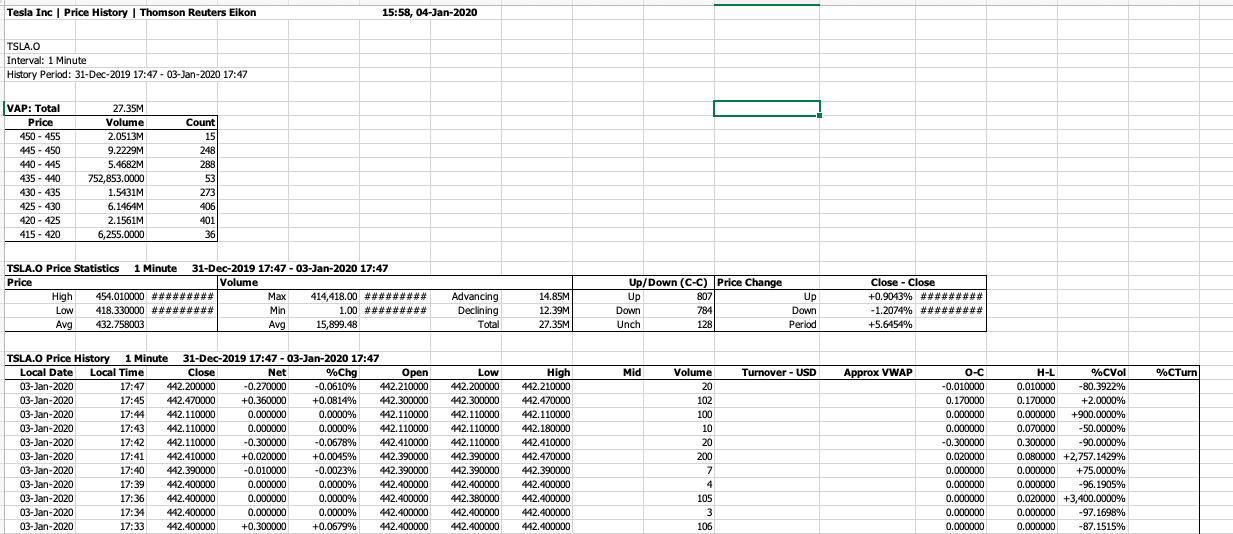
\includegraphics[width=17cm]{Chapters/Chapter_2_Section/Tesla_3_month_data.png}

    }
    
    \item Columns names\\
      \begin{itemize}
         \item Local Date
         \item Local Time 
         \item Close 
         \item Net 
         \item \%Chg
         \item Open 
         \item Low 
         \item High 
         \item Mid 
         \item Volumn 
         \item Turnover - USD 
         \item Approx VWAP
         \item O-C
         \item H-L
         \item \%CVol
         \item \%CTurn
         
         
         
 
      \end{itemize}
    
    
    
\end{enumerate}
\section{From Professor}
 
\begin{enumerate}
 
        \item\textbf{Bryan Kelly} \\
        \url{https://www.bryankellyacademic.org} 
        
        \item\textbf{Dacheng Xiu} \\
        \url{https://dachxiu.chicagobooth.edu} 
        
        \item\textbf{Stefan Nagel} \\
        \url{https://voices.uchicago.edu/stefannagel}  
        
        \item\textbf{Take a look at their recent research papers (which you can find in their webpages, under "research"), to get some basic ideas? (If the papers are hard to understand, that's all right. You just need to get some basic "feeling" at this point.) } 
         
  
        \item\textbf{Stefan Nagel - A nice tutorial on ML for asset pricing } \\
        \url{https://bcf.princeton.edu/wp-content/uploads/2019/05/PrincetonLecturesSlides_Day1_handouts.pdf} 
   
\end{enumerate}


 
\chapter{Research Progress}\label{chapter:Research Progress}
This chapter main elaborate the research progress about machine learning applications in economics and finance

\section{Week 1 (Dec 22 - Dec 27)}
 
\begin{enumerate}
 
        \item\textbf{Bryan Kelly} \\
        \url{https://www.bryankellyacademic.org} 
        
        \item\textbf{Dacheng Xiu} \\
        \url{https://dachxiu.chicagobooth.edu} 
        
        \item\textbf{Stefan Nagel} \\
        \url{https://voices.uchicago.edu/stefannagel}  
        
        \item\textbf{Take a look at their recent research papers (which you can find in their webpages, under "research"), to get some basic ideas? (If the papers are hard to understand, that's all right. You just need to get some basic "feeling" at this point.) } 
         
  
        \item\textbf{Stefan Nagel - A nice tutorial on ML for asset pricing } \\
        \url{https://bcf.princeton.edu/wp-content/uploads/2019/05/PrincetonLecturesSlides_Day1_handouts.pdf} 
   
\end{enumerate}


\section{Week 2 (Dec 28 - Jan 4)}
\begin{enumerate}
    \item{Dive into paper "High-Frequency Factor Models and Regressions" 
        \begin{itemize}
         \item Un-systematic Risk (individual firm risk): Random events such as CEO step down, company being prosecuted, company news, etc; Systematic Risk (market wide risk): nationally cut interests rate, etc; 
         \item When portfolio size increase, the volatility will decrease because "Unsystematic Risk" averaging out.
         \item Total Risk = Systematic Risk + Unsystematic Risk
         \item How to measure Systematic risk? Beta
         \item Beta = the percentage change in an asset's return GIVEN a 1\% change in the market portfolio (market portfolio = all firms) - how individual return tied to market portfolio change
        \end{itemize}
        
    \item{Data from Thomson Reuters}
        \begin{itemize}
            \item Login Page:
                \begin{itemize}
                    \item  \url{https://php.library.tamu.edu/resources/datastream/} or 
                    \item  \url{http://eikon.thomsonreuters.com/login}
                \end{itemize}
            \item Credentials: 
                \begin{itemize}
                    \item   Account: student3@tamu.edu  | Password: TAMUwcl1
                    \item   Account: student2@tamu.edu  |Password: WCLtamu1
                    \item   Account: student1@tamu.edu  | Password: WCLtamu1
                \end{itemize}

        \end{itemize}
    
      \item{Data from Eikon Data API}
        \begin{itemize} 
           \item eikon PyPI  \url{https://pypi.org/project/eikon/}
           \item Quick Start  \url{https://developers.refinitiv.com/eikon-apis/eikon-data-api/quick-start}
           \item Tutorials
           \url{https://developers.refinitiv.com/eikon-apis/eikon-data-api/learning}
        \end{itemize}
        
     \item Sample Minutes Price (3 months) \\
            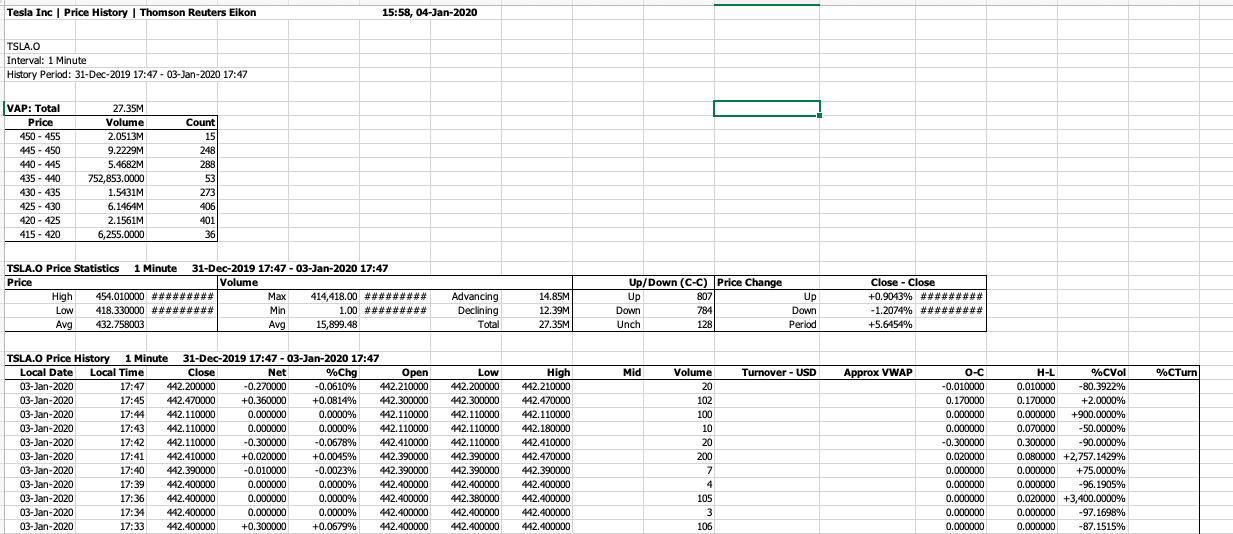
\includegraphics[width=17cm]{Chapters/Chapter_2_Section/Tesla_3_month_data.png}

    }
    
    \item Columns names\\
      \begin{itemize}
         \item Local Date
         \item Local Time 
         \item Close 
         \item Net 
         \item \%Chg
         \item Open 
         \item Low 
         \item High 
         \item Mid 
         \item Volumn 
         \item Turnover - USD 
         \item Approx VWAP
         \item O-C
         \item H-L
         \item \%CVol
         \item \%CTurn
         
         
         
 
      \end{itemize}
    
    
    
\end{enumerate}

\section{Week 3 (Jan 5 - Jan 11)}
\section{Week 4 (Jan 12 - Jan 18)}
 

\chapter{Terminology}\label{chapter:Terminology}
\begin{enumerate}
    
        \item\textbf{Book-To-Market Ratio Definition} \\     \url{https://www.investopedia.com/terms/b/booktomarketratio.asp}

        \item\textbf{Price-to-Book ratio, or P/B ratio} \\
        \url{https://en.wikipedia.org/wiki/P/B_ratio}

        \item\textbf{Market to Book Ratio} \\
        \href{https://www.youtube.com/watch?v=aPoHIdaMPuI}{Reference Link 1} 
 
        \item\textbf{Fama French Three Factors Model}  \\ 
          \href{https://www.youtube.com/watch?v=qeNBAKtAIHo}{Reference Link 1} \\
          \href{https://www.youtube.com/watch?v=pYTraS5WR3s&list=PLsJJSEojXyUHWidbRoBGR0mBgEkXVAkKM&index=2&t=0s}{Reference Link 2} 
  
        \item\textbf{Arbitrage} \\ 
          \url{https://www.investopedia.com/terms/a/arbitrage.asp}
         
        \item\textbf{Near-Arbitrage} \\
          \url{http://people.stern.nyu.edu/adamodar/pdfiles/invphilslides/session28.pdf}
          
        \item\textbf{Sharpe Ratios} \\
        \url{https://www.investopedia.com/ask/answers/010815/what-good-sharpe-ratio.asp} \\
        \href{https://www.zhihu.com/question/264210987}{Reference Link 2} \\
        \href{https://www.youtube.com/watch?v=fWnyg0UeQkg}{Reference Link 3} 
            
        \item\textbf{Factor Return} \\ 
        \url{https://www.nasdaq.com/glossary/f/factor-return} 
   
        \item\textbf{Hansen-Jagannathan Distance:  Geometry and Exact Distribution} \\
        \url{Hansen-Jagannathan Distance:  Geometry and Exact Distribution} 
        
        \item\textbf{Stochastic discount factor}\\
        \href{https://en.wikipedia.org/wiki/Stochastic_discount_factor}{Reference Link 1}
        \href{https://www.youtube.com/watch?v=kHSNu6sfrfM}{Reference Link 2}
         
        \item\textbf{Hansen–Jagannathan bound}
        \url{https://en.wikipedia.org/wiki/Hansen%E2%80%93Jagannathan_bound}
        
        \item\textbf{Non-parametric Time Series Regression Model}
        
        \item\textbf{Local martingale} \\ 
        \url{https://en.wikipedia.org/wiki/Semimartingale}
        
        \item\textbf{Semimartingale} \\
        \url{https://en.wikipedia.org/wiki/Local_martingale}
        
        \item\textbf{Linear Conditional Beta Specification}
        \url{}
        
        \item\textbf{Book-to-Market}\\
        \url{https://www.investopedia.com/terms/b/booktomarketratio.asp}




\end{enumerate}

     
\section{Economics and Finance}
\section{Neural Network}

\chapter{Milestones}\label{chapter:Milestones}
This Chapter marks down the major progress and important finding etc.




\section{Before 2019/12}
\begin{enumerate}

    \item{Replicated and improved below LTMS project
    \begin{itemize}
    
  
    \item \url{https://github.com/zebointexas/LSTM-Neural-Network-for-Time-Series-Prediction}
    
    \item Conducted experiments for Apple Inc. 's 2009-2018 price in NSDAQ, archived 75\% accuracy when testing the result in 2019 
    
    \end{itemize}
    }
    
    
    
    
    \item{Data Collection 
    \begin{itemize}
      \item Be able to collect seconds data via Robinhood (every three seconds) by developing with Robinhood API.
      \item Be able to collect minutes data from Bloomberg for lag 3. 
      \item Be able to collect news, time series, constituents from Eikon by using Eikon library 
    
    \end{itemize}
    }
\end{enumerate}

 
\section{After 2019/12} 
\input{Chapters/Chapter_4_Section/Section_After_2019_Dec.tex}

\chapter{Previous \& Parallel Works}\label{chapter:Parallel Works}
\input{Chapters/Chapter5.tex}

\section{Video Steam Vehicle Data Extraction (Parallel)}
\begin{enumerate}

    \item{Replicated the project and attempting optimize the algorithm: \\ \url{h^^s://github.com/ahmetozlu/vehicle_counting_tensorflow}  }  
 
    \item{ __  \\
     
            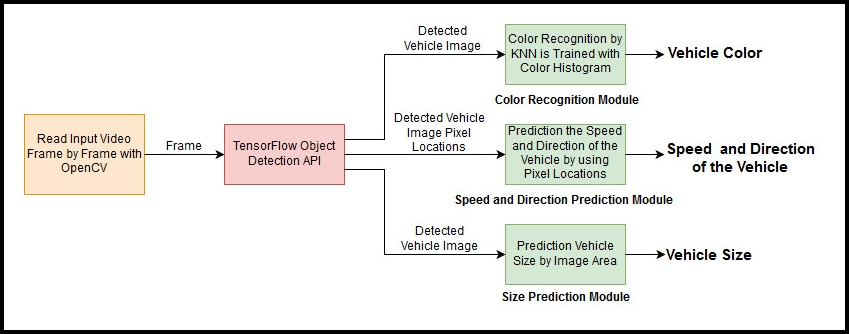
\includegraphics[width=10cm]{Chapters/Chapter_5_Section/System_Architecture.jpg}
  
    }
 
\end{enumerate}


    

\section{LSTM for Time Series Prediction (Previous)}
\begin{enumerate}

    \item{Replicated and improved below LTMS project
    \begin{itemize}
    
  
    \item \url{https://github.com/zebointexas/LSTM-Neural-Network-for-Time-Series-Prediction}
    
    \item Conducted experiments for Apple Inc. 's 2009-2018 price in NSDAQ, archived 75\% accuracy when testing the result in 2019 
    
    \end{itemize}
    }
    \item {Sequential by Sequential prediction (4 Epoch, 50 Batch size)
    
      \\
     
            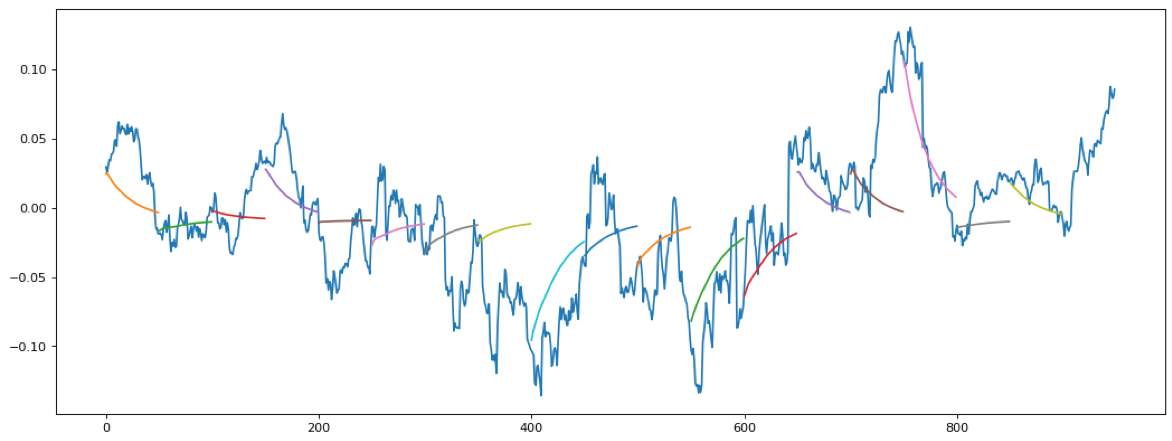
\includegraphics[width=10cm]{Chapters/Chapter_5_Section/SS_4_50.png}
            
         
 
    }
    
  \item { Point-by-Point prediction (8 Epoch, 50 Batch size)
    
      \\
     
          
            
            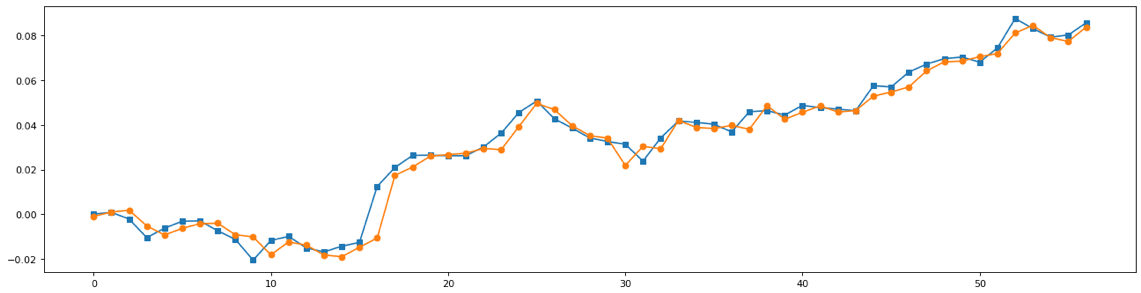
\includegraphics[width=10cm]{Chapters/Chapter_5_Section/PP_8_50.png}
 
    }
    
\end{enumerate}    

\section{On-Off Campus Ride Sharing Platform (Parallel)}
\begin{enumerate}

\item{Built a responsive web platform with Django/Bookstrap/MySQL to help students post rides information.}
 
 
\item{ Utilized GitHub and deployed the project on PythonAnywhere server for public testing.}

\item{ Fine tuned and validated the front-end to meet requirements such as intelligent rides recommendation. }
 
 
\end{enumerate}

\section{Facial Recognition \& Django Development (Previous)}
\begin{enumerate}

\item{
 Developed a Twitter like social medial platform with Django which gives object and face recognition on the images uploaded for privacy protection purpose;}
 
\item{Incorporated OpenCV and Google Cloud Vision and Python face recognition package into the platform to process the image detection.}

\item{Designed and adapted machine learning algorithm with Python to train models for better detection (such as language characters and indoor objections) optimization.} 
 
 
 \end{enumerate}

\section{Software Engineering - Program Invariants Detection (Previous)} 
\begin{enumerate}
    
        \item{
         Utilized Daikon software and Symbolic Execution techniques to generate candidate invariants and implemented selfdesigned algorithms to produced better invariants set.}  
     
         \item{Configured and deployed Java/Symbolic PathFinder on Unix environment with Gradle and Eclipse; Employed Homebrew to setup prerequisites such as Graphviz, Texinfo, GNU Compiler Collection (GCC) to support invariants discovery.}
 
 \end{enumerate}

\section{2019 Fall Class Summary (Previous)} 
\begin{enumerate}
    \item{\mathbf{CSCE 676 – Data Mining and Analysis (Dr. James Caverlee)}  
    \begin{itemize}
       \item Generated association rules (support >=minsup, confidence >= minconf) using hash-based Apriori to generate the rules)
        \item Ranked the graph nodes using the Personal Page Ranking 
        \item Performed Text Mining, Sentimental Analysis, Topic Modelling, Expectation Maximization on millions of text file crawled from Google regarding corporate social responsibilities 
        \item Understood MapReduce programming model; Studied the concepts in Hadoop; Analyzed the tweets concerning members of the US congress (such as most mentioned users) on AWS using Spark with Pregel 
        \item Performed K-means for different clusters; Hierarchical clustering (single link & complete link) 
        \item Tufte's Principles (such as maximizing the data-ink ratio & erasing redundant data-ink)
        \item Finding similarities using Jaccard distance with shingling, min-hashing, and locality-sensitive hashing (LSH) 
        \item Understood consistent hashing on Napster; Studied structured P2P approaches such as Chord using Finger table; Used counting bloom filter algorithm to test whether a movie is a member of a set;  
        \item Used Reservoir sampling in data stream; Adopted Morris algorithm and Flajolet-Martin algorithm to perform probabilistic counting 
        \item Studied Privacy-Preserving data mining for association rule mining, k-means clustering, and decision trees.  
        \item Used K-anonymity to remove personally identifying information; Understood differential privacy;  
 
    \end{itemize}
    
  \item{\mathbf{CSCE 633 – Machine Learning (Dr. Bobak Mortazavi) }  
    \begin{itemize}
       \item Studied multiple linear regression with model fitting; Understood the concept of convexity;   \item Studied multiple logistic regression and perform optimization using cross-entropy (gradient descent with different learning rate) 
       \item Performed model selection with lasso(L2) and ridge(L1) regression  
       \item Studied SVM using hyperplane to classify the data; several techniques are: 1) maximal marginal hyperplane; 2) Enlarge through kernel space; 3) Adopted Hinge Loss and Lagrange Multipliers 
       \item Studied decision tree and used Gini Index to avoid overfitting; Studied random forests and AdaBoost  
       \item Used PCA to reduce the dimension and K-Means to find patterns in clusters
       \item Studied Expectation Maximization to increase the likelihood   
       \item Studied neural network with the concepts of perceptron, forward/backward propagation calculation. \item Learnt how convolutional neural networks use kernels and max-pooling techniques.  
       \item Understood reinforcement learning and its Hidden Markov Model 
       \item Predicted NASDAQ price with LSTM (RNN) using Keras API and archived 75% up/down prediction accuracy. (Hourly data from 2009 to 2019) 
    \end{itemize}
    
    
  \item{\mathbf{ CSCE 636 Deep Learning (Dr. Shuiwang Ji)   
       \begin{itemize}
       \item Studied the concept of Perceptron, threshold and Perceptron Learning Algorithm (PLA).   
       \item Studied linear classification, Pocket Algorithm, Least Squares Linear Regression. 
       \item Adopted Cross Entropy and maximized the likelihood to minimize the total error using Stochastic Gradient Descent.  
       \item Calculated probability for multi-class logistic regression using softmax; Measured the error using corss entropy to calculate individual class’s loss; Studied the shift-invariance in parameters (output remain the same); Studied the equivalence of sigmoid when cross entropy cope with binary classes;
       \item Calculated the derivative of software and derivative of cross entropy with softmax;
       \item Learnt different loss functions such as: Hinge Loss, Log Loss, Zero-one Loss; Studied convexity;  \item Studied how to use regularization (Lasso, Ridge), cross-validation and early stopping techniques to prevent overfitting during model selection;  
       \item Studied the multilayer perceptron (MLP) and the reason to use adopt tanh(.) activation function (original error is not smooth and cannot use gradient descent) 
       \item Utilized Chain Rule to produce sensitivities during the backpropagation process. 
       \item Compared different descents such as steepest descents, conjugate gradients, etc. 
       \item Understood thoroughly about SVD and its relation to Eigen-Decomposition; Learnt compact SVD; Learnt how to compute PCA and the reconstruction process; Studied Autoencoder; 
       \item Studied the concept of fully connected layer, filters, max-pooling, ReLU, stride and padding in CNN and how to calculate the output volume size;   
       \item Studied batch normalization and the suitable position to insert in CNN; Advantages such as improving gradient flow through the network, allowing higher learning rate and reducing the strong dependence on initialization;  
       \item Understood SGD with Momentum, second-order optimization; Understood model ensembles, dropout, data augmentation to prevent overfiting.
       \item Understood the concept of transfer learning;  
       \item Learnt different CNN such as AlexN;
       \item Calculated the loss in RNN Language Model and performed the backpropagation with multivariable chain rule;  
       \item Understood the vanishing and exploding gradient problem in RNN; Studied the architecture of LSTM; \item Understood the mechanism in Attention;  
       \item Knowledge in Graph Convolutional  Networks; Knowledge in graph pooling with clustering and its limitations;
    \end{itemize}}
\end{enumerate}



\bibliographystyle{unsrt}
\bibliography{References}
\newpage

\appendix
\addcontentsline{toc}{chapter}{Appendix}
\chapter{My First Appendix}\label{chapter:Appendix A}
In this file (Appendices/Appendix$\_$A.tex) you can add appendix chapters, just as you did in the Document.tex file for the `normal' chapters.
You can also choose to include everything in this single file, whatever you prefer.

\end{document}